% !TeX spellcheck = en_US
\newpage
\section{Prediction}
\subsection{Least Square Regression}
We build a \textbf{model} predicting $y$ from $x$:
\begin{equation}
	f(\mathbf{x}) = \mathbf{w}^\top\mathbf{x} + b
\end{equation}
and we find the model \textbf{parameters} so that prediction errors are minimized. An example could be to minimize the least squared error averaged over all instances:
\begin{equation}
	\min_{\mathbf{w},b} \mathbb{E}[(\mathbf{w}^\top\mathbf{x}+b-y)^2]
\end{equation}
\subsubsection{Centering}
To simplify regression we can \textbf{center} the data by putting $\mathbb{E}[\mathbf{x}] = \mathbf{0}$ and $\mathbb{E}[y]=0$. Then we can show that
\begin{equation}
	\arg \max_b \mathbb{E}[(f(\mathbf{x})-y)^2] = 0
\end{equation}
\begin{demonstration}
	\begin{equation*}
		\frac{\partial}{\partial b} \mathbb{E}[(f(\mathbf{x})-y)^2] = 2\mathbb{E}[(\mathbf{w}^\top\mathbf{x}+b-y)] \overset{\text{def}}{=} 0 \Rightarrow b=0
	\end{equation*}
	\hfill$\square$
\end{demonstration}
This implies that, without loss of accuracy, one can simplify the Least Square Regression problem as finding a homogeneous linear model that minimizes the square error:
\begin{equation}
	f(\mathbf{x}) = \mathbf{w}^\top\mathbf{x}
\end{equation}
\subsubsection{Linear regression}
We can develop it as:
\begin{align}
	\begin{split}
		\xi (\mathbf{w}) & = \mathbb{E}[(f(\mathbf{x}) -y)^2]\\
		& = \mathbb{E}[(\mathbf{w}^\top \mathbf{x}-y)^2] \qquad\qquad\qquad\quad \text{Substitution}\\
		& = \mathbb{E}[\mathbf{w}^\top \mathbf{x}\mathbf{x}^\top\mathbf{w}-2\mathbf{w}^\top\mathbf{x} y + y^2] \quad \text{Square calculation, n.b. } (\mathbf{w}^\top \mathbf{x})^2 = \mathbf{w}^\top \mathbf{x} \mathbf{x}^\top \mathbf{w}\\
		& = \mathbf{w}^\top C_{xx}\mathbf{w} - 2\mathbf{w}^\top C_{xy}+C_{yy} \qquad \text{Linearity and covariance definition}
		\label{eq:linregog}
	\end{split}
\end{align}
Since $C_{xx}$ is positive semi-definite, minimizing $\xi(\mathbf{w})$ is a \textbf{convex optimization problem} and the solution must necessarily have gradient zero:
\begin{equation}
	\nabla\xi(\mathbf{w}) = 2C_{xx}\mathbf{w} - 2C_{xy}=0 \longrightarrow \mathbf{w} = C_{xx}^{-1}C_{xy}
\end{equation}
If we inject this into the objective we get the \textbf{mean square error} at the optimum:
\begin{equation}
	\xi = C_{yy} - C_{yx}C^{-1}_{xx} C_{xy} \label{eq:linreg}
\end{equation}

\paragraph{Non-Invertible $C_{xx}$}
\begin{wrapfigure}[6]{r}{4cm}
\vspace{-.9cm}
\begin{center}
	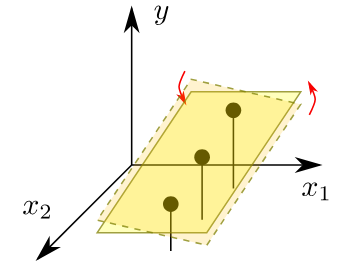
\includegraphics[width=4cm]{lsr}
\end{center}
\end{wrapfigure}
If we have $C_{xx}$ non invertible corresponds to the case  where the data only spans a subspace of $\mathbb{R}^d$. In this case, there are infinitely many possible solutions to the regression problem.\\
To solve this we virtually add some \textbf{noise} $\mathbf{n}$ to the data (adding a diagonal term to the covariance matrix) so that the covariance matrix is now invertible and favors solutions that are flat on directions that are orthogonal to the data.
\begin{align}
	\begin{split}
		C_{xx}^{\text{new}} & = \text{Cov} ( \mathbf{x}+\mathbf{n}, \mathbf{x} + \mathbf{n}) \\
		& = \text{Cov}(\mathbf{x}, \mathbf{x}) + 2 \text{Cov}(\mathbf{x}, m\mathbf{n}) + \text{Cov}(\mathbf{n}, m\mathbf{n})\\
		& = C_{xx}+\sigma_n^2I
	\end{split}
\end{align}
Using the new covariance in the error function \ref{eq:linreg} yields:
\begin{align}
	\begin{split}
		\xi^{\text{new}}&=C_{yy}-C_{yx}(C_{xx}^\text{new})^{-1}C_{xy} \\
		& = C_{yy} - C_{yx}(C_{xx} + \sigma_n^2 I)^{-1}C_{xy} \\
		& = C_{yy} - C_{yx} \bigg(\sum_{j=1}^{d} u_j u_j^\top ( \lambda_j + \sigma_n^2)\bigg)^{-1}C_{xy} \\
		& = C_{yy} - \sum_{j} (C_{yx}u_j)^2 \frac{1}{\lambda_j+\sigma_n^2}
	\end{split}
\end{align}
The larger the noise we inject, the higher the error: wee need just enough to make $C_{xx}$ invertible.

\paragraph{High Dimensions} When $d$ is large, computing and inverting $C_{xx}$ can get really expensive. To manage this, we start from the formulation \ref{eq:linregog} and we assume that an optimal $\mathbf{w}$ is found in the span of the data and we express it as a linear combination of the data $\mathbf{w} = X \mathbf{\alpha}$, where $X$ is a matrix of size $d \times N$ containing the centered data:
\begin{align}
	\begin{split}
		\xi(\mathbf{\alpha}) & = \overbrace{\mathbf{\alpha}^\top X^\top}^{\mathbf{\alpha}^\top}C_{xx}\overbrace{X\mathbf{\alpha}}^{\mathbf{w}} - 2 \overbrace{\mathbf{\alpha}^\top X^\top}^{\mathbf{w}^\top}C_{xy}+C_{yy} \\
		& = \frac{1}{N}\mathbf{\alpha}^\top \underbrace{X^\top XX^\top X}_{Q_x^2}-\frac{2}{N}\mathbf{\alpha}^\top \underbrace{X^\top X}_{Q_x}Y+C_{yy}
	\end{split}
\end{align} 
Since matrices $Q_x^2$ and $Q_x$ are of size $N \times N$ there is no need to compute matrices of size $d \times d$ anymore. Since $\xi(\mathbf{\alpha})$ is convex, we can find the solution where the gradient $\nabla\xi(\mathbf{\alpha}) = \frac{2}{N}Q_x^2\mathbf{\alpha}-\frac{2}{N}W_x Y$is zero:
\begin{equation*}
	\mathbf{\alpha} = (Q_x^2)^{-1}Q_xY = Q_x^{-1}Y
\end{equation*}
And therefore we need to invert only a matrix of size $N \times N$. From this we can then recover the original weight parameter as:
\begin{equation}
	\mathbf{w} = X \mathbf{\alpha}
\end{equation}

\subsubsection{CCA}
Since in the case of linear regression the second modality is \textbf{univariate}, there is no direction to be found in the second modality ($w_y = 1$) and the CCA objective (\ref{eq:cca}) simplifies to:
\begin{equation}
	\rho = \frac{\mathbf{w}_x^\top C_{xy}}{\sqrt{\mathbf{w}^\top_x C_{xx}\mathbf{w}_xC_{yy}}} 
\end{equation}
which can then be reformulated as a constrained optimization problem:
\begin{equation}
	\max_\mathbf{w} \mathbf{w}_x^\top C_{xy} \qquad\text{such that}\qquad \mathbf{w}_x^\top C_{xx}\mathbf{w}_xC_{yy} = 1 \label{eq:ccalsr}
\end{equation}

\paragraph{Weights}
To derive the weights we solve the problem indicated in equation \ref{eq:ccalsr} with Lagrange's Multipliers:
\begin{align*}
	&\mathcal{L}(\mathbf{w}_x, \lambda) = \mathbf{w}_x^\top C_{xy} + \frac{1}{2} \lambda (1-\mathbf{w}_x^\top C_{xx}\mathbf{w}_x C_{yy}) \\
	&\frac{\partial \mathcal{L}}{\partial\mathbf{w}_x} = C_{xy}-\lambda C_{xx}\mathbf{w}_x C_{yy} = 0 \Longrightarrow \mathbf{w}_x = \lambda^{-1}C^{-1}_{xx}C_{xy}C_{yy}^{-1}
\end{align*}
Therefore, setting $\lambda$ in a way that the constraint is satisfied, we get:
\begin{equation}
	\mathbf{w}_x = \frac{C_{xx}^{-1}C_{xy}}{\sqrt{C_{yx}C_{xx}^{-1}C_{xy}C_{yy}}} \label{eq:ccalsrw}
\end{equation}
which is exactly the same direction as the weight of the linear model $\mathbf{w} = C_{xx}^{-1}C_{xy}$.
\paragraph{Objective} To derive the objective we evaluate the CCA objective equation with the solution \ref{eq:ccalsrw}. This gives us the \textbf{correlation coefficient}
\begin{equation*}
	\rho = \mathbf{w}_x^\top C_{xy} = \sqrt{C_{yx}C_{xx}^{-1}C_{xy}C_{yy}^{-1}}
\end{equation*}
From which we can measure the \textbf{explained variance}
\begin{equation}
	C_{yy}\rho^2 = C_{yx}C_{xx}^{-1}C_{xy} \label{eq:cca1}
\end{equation}
which compared to the error of linear regression \ref{eq:linreg} indicates that the CCA objective and Least Square Regression ar related: they form a composition of the total variance.
\begin{equation}
	C_{yy} = C_{yy}\rho^2 + \xi
\end{equation}
This means that maximizing the correlation with CCA and minimizing Square Error achieve both the same objective.

\subsection{Outliers}
Square errors may be very large for data points whose outputs strongly deviate from that of other data points. Those with large prediction errors may be treated as \textbf{outliers} so that the model can focus on the non-outlier part of the data. Reduced sensitivity to those can be achieved by considering absolute deviations instead of squared errors and invariance to small noise can be maintained by introducing a small \textbf{slack} $\epsilon$.
\begin{center}
	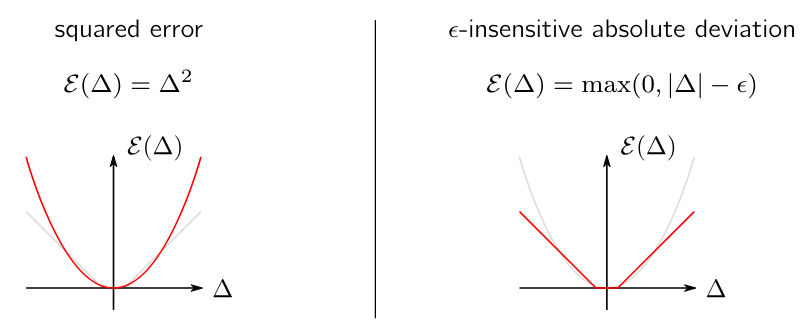
\includegraphics[scale=0.3]{regout}
\end{center}
To do this we replace the square error in the original problem by the $\epsilon$-insensitive absolute deviation and we add a \textbf{penalty term} $\lambda\lvert\lvert \mathbf{w}\rvert\rvert^2$ to favor the flattest solution:
\begin{equation*}
	\min_\mathbf{w} \mathbb{E}[(\mathbf{w}^\top \mathbf{x}-y)^2] \longrightarrow \min_{\mathbf{w},b}[\max(0,\lvert \mathbf{w}^\top x + b -y \rvert -\epsilon)] + \lambda\lvert\lvert \mathbf{w}\rvert\rvert^2
\end{equation*}
\begin{note}
	We have to reintroduce the bias $b$ because we are no longer guaranteed that a solution without it is optimal.
\end{note}

\subsubsection{Support  Vector Regression}
An algorithm that implements this is Support Vector Regression, which takes the form of a quadratic optimization problem with linear constraints. The \textbf{primal} version is:
\begin{align}
	\begin{split}
		\min_{\mathbf{w},b,\mathbf{\xi},\mathbf{\xi^\star}} \frac{1}{2}  \lvert\lvert \mathbf{w}\rvert\rvert^2+C\sum_{i=1}^{N}(\xi_i + \xi_i^\star) \qquad \text{such that} \qquad & \forall_{i=1}^N : \mathbf{w}^\top \mathbf{x}_i + b - y_i \leq \epsilon + \xi_i \\
		& \forall_{i=1}^N : y_i -\mathbf{w}^\top \mathbf{x}_i + b \leq \epsilon + \xi_i \\
		& \xi_i, \xi_i^\star \geq 0
	\end{split}
\end{align}
The \textbf{dual} version is:
\begin{align}
	\begin{split}
		\max_{\alpha, \alpha^\star} -\frac{1}{2}\sum_{ij}(\alpha_i-\alpha_i^\star)(a_j - a_j^\star)\mathbf{x}_i^\top \mathbf{x}_j  \qquad \text{such that} \qquad & \sum_i(a_i - a_i^\star) = 0 \\
		- \varepsilon \sum_i(a_i +a_i^\star) +\sum_i y_i(a_i - a_i^\star)  \qquad \qquad\qquad\qquad& a_i, a_i^\star \in [0, C]
	\end{split}
\end{align}
This algorithm enable the model to be robust to outliers data and to small noise perturbations. Both versions take the form of a quadratic optimization problem with linear constraints. The \textbf{disadvantages} are that SVR has no closed form solution and there is no simpler relation between the objective and statistical measures (e.g. correlation, variance).

\subsection{Difference of means}
Let $\mathbf{x}_1, \ldots, \mathbf{x}_n$ be a dataset and each member is an instance of one the two groups. Let $\mathcal{G}_1$ and $\mathcal{G}_2$ be the set instances of each group.\\
We formulate the problem of \textbf{discriminant learning} as finding a unit-norm vector $\mathbf{w}$ such that the projected data points are maximally different between the two groups on average:
\begin{align}
	\begin{split}
		\max_{\mathbf{w}} &\frac{1}{\lvert \mathcal{G}_1\rvert \lvert \mathcal{G}_2 \rvert} \sum_{i \in \mathcal{G}_1} \sum_{j \in \mathcal{G}_2} (\mathbf{w}^\top \mathbf{x}_i- \mathbf{w}^\top\mathbf{x}_j) \\
		& = \max_{\mathbf{w}} \frac{1}{\lvert \mathcal{G}_1\rvert \lvert \mathcal{G}_2 \rvert} \mathbf{w}^\top \bigg(\lvert \mathcal{G}_2\rvert\sum_{i \in \mathcal{G}_1} \mathbf{x}_i - \lvert \mathcal{G}_1 \rvert \sum_{j \in \mathcal{G}_2} \mathbf{x}_i\bigg) \\
		& = \max_{\mathbf{w}} \mathbf{w}^\top \bigg(\frac{1}{\lvert \mathcal{G}_1\rvert}\sum_{i \in \mathcal{G}_1} \mathbf{x}_i - \frac{1}{\lvert \mathcal{G}_2 \rvert }\sum_{j \in \mathcal{G}_2} \mathbf{x}_i\bigg) \\
		& = \max_{\mathbf{w}} \mathbf{w}^\top (\mu_1 - \mu_2)
	\end{split}
\end{align}
and the unit-norm vector $\mathbf{w}$ that maximizes this objective is the difference of means:
\begin{equation}
	\mathbf{w} = \frac{(\mu_1 -\mu_2)}{\lvert\lvert \mu_1-\mu_2\rvert\rvert}
\end{equation}
\subsubsection{Fisher Discriminant}
Sometimes a better model can be achieved by rotating the projection, increasing their \textbf{separability}.
\begin{center}
	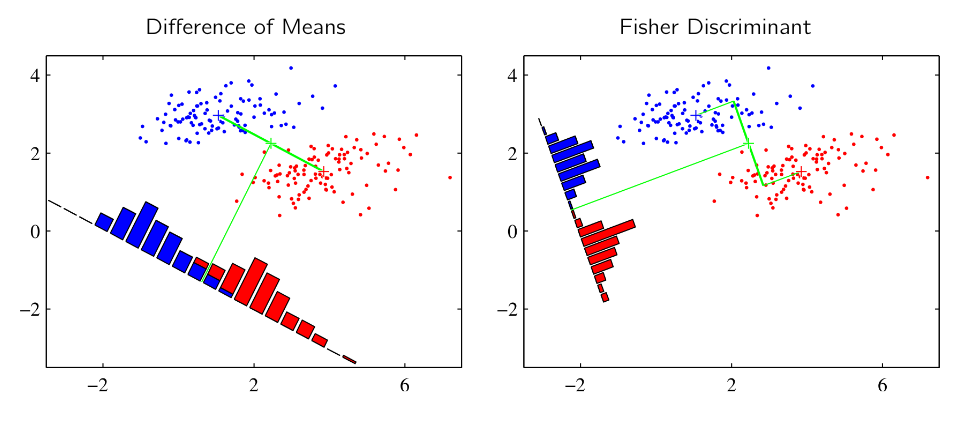
\includegraphics[scale=.4]{fischer}
\end{center}
To do this, in addition to maximizing the separation between class means in projected space, the Fisher Discriminant also \textbf{reduces the within group scatter}:
\begin{equation}
	s_k(\mathbf{2}) = \sum_{i \in \mathcal{G}_k} (\mathbf{w}^\top (\mathbf{x}_i - \mu_k))^2
\end{equation}
Then we define the new \textbf{objective} as:
\begin{equation}
	\max_{\mathbf{w}} \frac{\mathbf{w}^\top (\mu_1 - \mu_2)}{\sqrt{s_1(\mathbf{w}) + s_2(\mathbf{w})}}
\end{equation}
Since the \textbf{scatter terms} have the quadratic form
\begin{equation*}
	s_k(\mathbf{w}) = \mathbf{w}^\top \underbrace{\sum_{i \in \mathcal{G}_k} (\mathbf{x}_i - \mu_k) (\mathbf{x}_i - \mu_k)^\top\mathbf{w}}_{S_k}
\end{equation*}
we can rewrite the objective as
\begin{equation}
	\max_{\mathbf{w}} \frac{\mathbf{w}^\top (\mu_1 - \mu_2)}{\sqrt{\mathbf{w}^\top (S_1 + S_2) \mathbf{w}}}
\end{equation}
and since the objective is invariant to a rescaling of $\mathbf{w}$, we can use instead this constrained optimization problem:
\begin{equation}
	\max_{\mathbf{w}} \mathbf{w}^\top (\mu_1 - \mu_2) \qquad \text{such that} \qquad \frac{1}{2} \mathbf{w}^\top (S_1+ S_2) \mathbf{w} = 1
\end{equation}
Which can then be solved with the Lagrange's Multipliers method:
\begin{equation*}
	\mathbf{w} = (S_1 + S_2)^{-1}(\tau_1 - \tau_2)
\end{equation*}
\paragraph{Connection to CCA}
The Fisher Discriminant  can be seen as a special case of CCA: interpretation as a projection that maximizes correlation between input and output. To demonstrate this we develop the cross-covariance between $\mathbf{x}$ and $y$  as:
\begin{align*}
	C_{xy} & = \frac{1}{N} \sum_{i=1}^{N} (\mathbf{x}_i -\mu_x)(y_i - \mu_y) \\
	& = \frac{1}{N} \bigg[\sum_{i \in \mathcal{G}_1}(\mathbf{x}_i -\mu_x)(1 - \mu_y) + \sum_{i \in \mathcal{G}_2}(\mathbf{x}_i -\mu_x)(-1 - \mu_y)\bigg] \\
	& = \frac{1}{N} \bigg[\sum_{i \in \mathcal{G}_1}(\mathbf{x}_i -\mu_x) - \sum_{i \in \mathcal{G}_2}(\mathbf{x}_i -\mu_x) + \underbrace{\sum_{i=1}^{N}(\mathbf{x}_i - \mu_x)}_0 \cdot (-\mu_y)\bigg] \\
	& = \frac{\lvert \mathcal{G}_1 \rvert}{N} (\mu_1 -\mu_x) - \frac{\lvert \mathcal{G}_2\rvert}{N}(\mu_2 - \mu_x) \\
	& = \frac{2\lvert\mathcal{G}_1\rvert\lvert \mathcal{G}_2\rvert}{N^2}(\mathcal{\mu}_1 - \mu_2)
\end{align*}
and since $y$ follows essentially a Bernoulli distribution, we get:
\begin{equation}
	C_{yy} = \frac{4\lvert\mathcal{G}_1\rvert\lvert \mathcal{G}_2\rvert}{N^2}
\end{equation}
We can the inject these two found covariances into \ref{eq:cca1} and we get:
\begin{align*}
	\rho^2 & = C_{yx}C_{xx}^{-1}C_{xy}C_{yy}^{-1}\\
	& = \frac{2\lvert\mathcal{G}_1\rvert\lvert \mathcal{G}_2\rvert}{N^2}(\mu_1 - \mu_2)C_{xx}^{-1}\frac{2\lvert\mathcal{G}_1\rvert\lvert \mathcal{G}_2\rvert}{N^2}(\mu_1 - \mu_2)\frac{N^2}{4\lvert\mathcal{G}_1\rvert\lvert \mathcal{G}_2\rvert} \\
	& = \frac{\lvert\mathcal{G}_1\rvert\lvert \mathcal{G}_2\rvert}{N^2}(\mu_1 - \mu_2)^\top C_{xx}^{-1}(\mu_1 - \mu_2)
\end{align*}
and substituting to \ref{eq:ccalsrw} we get
\begin{align*}
	\mathbf{w}_x & = \frac{C_{xx}^{-1}C_{xy}}{\sqrt{C_{yx}C_{xx}^{-1}X_{xy}}} \\
	& = \frac{C_{xx}^{-1}\frac{2\lvert\mathcal{G}_1\rvert\lvert \mathcal{G}_2\rvert}{N^2}(\mu_1 - \mu_2)}{\sqrt{\ldots}}\\
	& \propto C_{xx}^{-1}(\mu_1 - \mu_2)
\end{align*}
\begin{proposition}
	CCA and the Fisher vector point to the same direction
	\begin{equation}
		(S_1 + S_2)^{-1}(\mu_1 - \mu_2) \propto C_{xx}^{-1}(\mu_1 - \mu_2)
	\end{equation}
\end{proposition}
\begin{demonstration}
	\begin{align*}
		C_{xx} & = \frac{1}{N} \sum_{i=1}^{N} (x_1 - \mu)(\mathbf{x}_i - \mu)^\top \\
		& = \frac{1}{N} \sum_{k \in \{1,2\}}\sum_{i \in \mathcal{G}_k} (\mathbf{x}_i - \mu) (\mathbf{x}_i \mu)^\top \\
		& = \frac{1}{N} \sum_{k \in \{1,2\}}\sum_{i \in \mathcal{G}_k} (\mathbf{x}_i -\mu_k + \mu_k -\mu)(\mathbf{x}_i - \mu_k + \mu_k -\mu)^\top \\
		& = \bigg(\frac{1}{N} \underbrace{\sum_{k \in \{1,2\}}\sum_{i \in \mathcal{G}_k} (\mathbf{x}_i-\mu_k)(\mathbf{x}_i - \mu_k)^\top}_{S_1 + S_2}\bigg) + \alpha \cdot (\mu_1 - \mu_2)(\mu_1 - \mu_2)^\top + 0
	\end{align*}
	Then, using the identity $(A + \mathbf{b}\mathbf{b}^\top)^{-1} \mathbf{b} \propto A^{-1}\mathbf{b}$ we get that
	\begin{equation*}
		C_{xx}^{-1}(\mu_1 - \mu_2) \propto (S_1 + S_2)^{-1} (\mu_1 - \mu_2)
	\end{equation*}
	\hfill $\square$
\end{demonstration}

\subsection{Support Vector Machine}
Fisher Discriminant is \textbf{strongly affected} by the presence of \textbf{outliers} and may underestimate how predictable group membership is. To solve this problem, we focus on the \textbf{separation between the two groups} rather than their distribution and implement a mechanism that's robust to outliers.\\

To do that we learn a \textbf{hyperplane} that separates the two groups, called the \textbf{Perceptron}. Among all hyperplanes, the SVM chooses the one with the largest margin from the data points.\\
The SVM penalizes absolute deviations instead of square errors to allow for outliers. Therefore, the optimization problem (\textbf{primal problem}) is:
\begin{equation}
	\min_{\mathbf{w},b, \xi} \frac{1}{2} \lvert\lvert \mathbf{w} \rvert\rvert ^2 + C \sum_{i=1}^{N} \xi_i \qquad\text{such that} \qquad \forall_{i=1}^N : (\mathbf{w}^\top \mathbf{x}_i+b) \cdot y_i \geq 1-\xi_i \qquad \xi_i \geq 0
\end{equation}

\subsubsection{Dual problem}
When $d\gg N$ we can use the dual formulation:
\begin{equation}
	\max_\alpha \sum_{i=1}^{N}\alpha_i - \frac{1}{2} \sum_{i=1}^{N} \sum_{j=1}^{N} \alpha_i \alpha_jy_iy_j\mathbf{x}_i^\top \mathbf{x}_j \qquad \text{such that} \qquad \sum_{i}\alpha_i y_i = 0 \qquad \alpha_i \in [0, C]
\end{equation}
\subsubsection{Pros and cons}
SVM has a \textbf{better separation of groups} that Fisher discriminant for general data, it's more \textbf{robust to outliers} enabled by slack variables $\xi_i$ and has a \textbf{convex formulation}, meaning that is guaranteed to converge to the minimum of the objective.\\

On the other hand is \textbf{less suitable} than Fisher Discriminant if we care about within-group homogeneity in projected space, has \textbf{no closed-form solution} and it's not connected to CCA, meaning there is \textbf{no interpretation as maximizing correlation}.